\documentclass[11pt]{article}
\usepackage{tikz}
\usetikzlibrary{arrows}
\usetikzlibrary{shapes}
\usepackage{pgfmath}
\usepackage{setspace}
\usepackage{amsmath}
\usepackage{array}
\usepackage{hyperref}
\usepackage{enumerate}
\usepackage{enumitem}
\setlist{noitemsep}
\usepackage{listings}
\lstset{language=python}
\usepackage{makeidx}
\usepackage{verbatim}
\usepackage{datetime}

\setlength{\pdfpageheight}{11in}
\setlength{\textheight}{9in}
\setlength{\voffset}{-1in}
\setlength{\oddsidemargin}{0pt}
\setlength{\marginparsep}{0pt}
\setlength{\marginparwidth}{0pt}
\setlength{\marginparpush}{0pt}
\setlength{\textwidth}{6.5in}

%\usepackage[notes,backend=biber,isbn=false]{biblatex-chicago}
\usepackage[
	backend=biber,
	style=alphabetic,
	citestyle=ieee
]{biblatex}
\addbibresource{../../Accident_Analysis_and_Prevention/Accident_Analysis_and_Prevention.bib}
\AtEveryBibitem{\clearfield{note}\clearfield{addendum}}
\AtEveryCitekey{\clearfield{note}\clearfield{addendum}}

\pagestyle{plain}
\makeindex

\title{24 May 2021 Report}
\author{Brad Burkman}
\newdateformat{vardate}{\THEDAY\ \monthname[\THEMONTH]\ \THEYEAR}
\vardate
\date{\today}

\begin{document}
\setlength{\parindent}{20pt}
\begin{spacing}{1.2}


\maketitle
\tableofcontents

%%%%%
\section{Progress}

Besides the things below, I reviewed more {\it AA\&P} articles, and read the two articles in the \hyperref[sec:references]{References}.  Reading the articles is slow, because I'm taking notes on, and looking up, things I don't understand.  

%%%%%
\section{Jargon to Understand}

\begin{itemize}
	\item Naturalistic Driving Data - Data collected from sensors installed in the driver's own car, trying to get as close as possible to the driver's ``natural'' behavior.
	\item Heterogeneity.  I understand vaguely what ``data heterogeneity'' means, but I'm going to watch for the term to see how it's used in the context of these papers.  
\end{itemize}

%%%%%
\section{IRB, SHRP Database}

Eleven of the papers in {\it Accident Analysis and Prevention} used the Strategic Highway Research Program 2 (SHRP2) Naturalistic Driving Study (NDS), which put sensors in 3400 cars and recorded five million trips, including crashes.  To get ``Qualified Researcher Status'' with ``full access to data that has been made available through the SHRP 2 NDS Data Access Website,'' I had to submit a certificate of training on research with human subjects.  I did the training through the UL Institutional Review Board (IRB). I now have access.  

%%%%%
\section{NGSIM Database}

Three papers use the Next Generation Simulation dataset from the US Dept of Transportation, and it's available for download with no restrictions.  

%%%%%
\section{Mining Bibliographies}

There's an open-source project called  \href{https://github.com/inukshuk/anystyle}{Anystyle}.  If you have a folder with (hundreds, thousands) of PDF files, Anystyle will extract the {\it References} sections of all of the files as a Bib\TeX \ file.  

I have a file of the 190 articles from {\it Accident Analysis and Prevention} that I've reviewed.  I used Anystyle to extract the  references, and converted it to a Pandas dataframe.  Of the 10,822 references, 8,685 are unique.  Most interesting is to find the most-cited articles.  Seventeen of the 190 articles cited Mannering's 2016 article.  

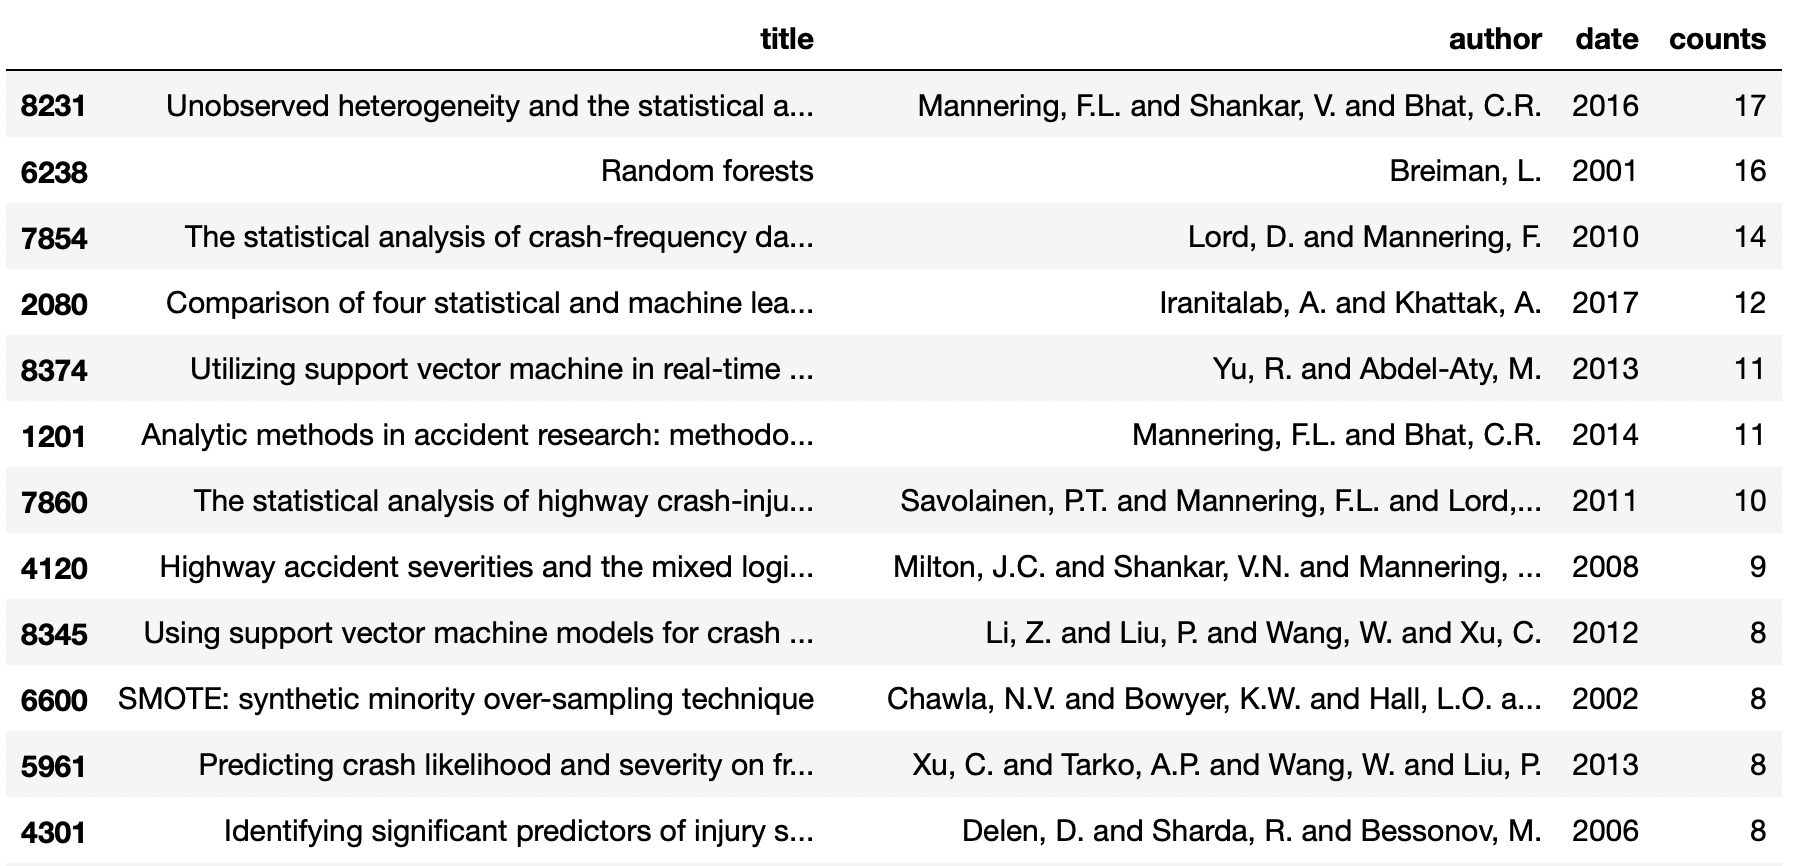
\includegraphics[width=\linewidth]{Screen Shot 2021-05-24 at 6.35.11 AM.png}

I had to spend some time playing with the arguments, because default Anystyle doesn't handle two-column PDF files well.

%%%%%
\section{Ideas for a Paper}

%%%
\subsection{Comparing Image Transformation Techniques}

In ``A deep learning based traffic crash severity prediction framework'' by Rahim (LSU) \cite{RAHIM2021106090}, they transformed each data point into an image, and used the images as input for a Convolutional Neural Network (CNN) for classification.  There are several ways to make such a transformation.  Write a paper where I compare different image transformation methods, and their effect on different metrics (precision, recall, accuracy, sensitivity, f1, false alarm rate) of the classification of the test set.  

%%%
\subsection{Comparing Data Cleaning Techniques}

In ``A deep learning based traffic crash severity prediction framework'' by Rahim (LSU) \cite{RAHIM2021106090}, they just deleted any records with missing or inconsistent data.  The {\it Titanic} Kaggle sites you showed me use several other methods for filling in incomplete data.  Write a paper where I compare different methods for dealing with missing data, and their effect on different metrics (precision, recall, accuracy, sensitivity, f1, false alarm rate) of the classification of the test set.  

Rahim's article took out 37\% of the records for missing or inconsistent data, but only 21\% of the fatal crashes; could that imbalance in the data cleaning skew the model prediction?  It makes sense that police would be more meticulous in their record keeping for fatal crashes, but 21\% and 37\% are huge.  

Would we get a better model if we found a good way to fill in missing data?

%%%
\subsection{Missing Data Analysis}

This isn't a ML paper, but somebody should write it.  In what situations is the crash data most likely to be incomplete or inconsistent?  Rather than a, ``How can we fix the roads to make them safer?,'' this would be a ``How can we get better records, so we can know how to fix the roads to make them safer?''

%%%
\subsection{Fill Holes in Osman et al}

A group at LSU has a 2019 paper \cite{OSMAN2019274} using the SHRP-2 data to predict, based on the driving behavior whether the driver was making a phone call, texting, or having a conversation with a passenger, but ``the effect of roadway and geometric characteristics is not within the scope of this paper.''  They say that in the introduction and devote the entire last paragraph of the conclusion to laying out that hole that needs to be filled.  

The data is not just crashes, but any time a person was using a phone, texting, or talking.  

%%%
\section{References}
\label{sec:references}
\printbibliography[heading=none]




%%%%%%%%%%%%%%%%%%
% Index
%\clearpage
%\addcontentsline{toc}{section}{Index}
%\printindex

%%%%%%%%%%%%%%%%
\end{spacing}
\end{document}

%%%%%%%%%%%%
% Useful tools
%%%%%%%%%

\begin{lstlisting}
Put your code here.
\end{lstlisting}

\lstinputlisting[language=python]{source_filename.py}


